% ----------------------------------------------------------
% Desenvolvimento
% ----------------------------------------------------------
\chapter{Desenvolvimento}
\label{cap:desenvolvimento}
% ----------------------------------------------------------

Este capítulo apresenta como a ferramenta foi desenvolvida, e descreve a arquitetura de software utilizada, assim como bibliotecas e técnicas de programação. Este capítulo está organizado da seguinte forma : A seção \ref{sec:impl} descreve 



\section{Implementação}\label{sec:impl}

    A ferramenta foi desenvolvida utilizando a linguagem de programação JavaScript, com foco na orientação a objetos, com auxílio de HTML5 e CSS para a sua apresentação visual. A aplicação ocorre completamente no front-end e não possui partes executadas em servidor. Também não foi utilizado nenhum tipo de framework para auxiliar a organização do código. Além dessas ferramentas, foi utilizada a biblioteca JavaScript Cytoscape.

    A biblioteca Cytoscape é utilizada para manipulação de desenhos em HTML5, com foco na visualização de grafos, e foi escolhida pois é totalmente open source, e grafos são a forma mais comum de representação de autômatos, utilizada, por exemplo, no livro didático \cite{vieira2006}. A biblioteca foi utilizada apenas para o desenho dos grafos, tendo toda a parte de simulação de autômatos sido desenvolvida durante este trabalho. O codigo fonte está disponível no GitHub e o software está hospedado de forma gratuita por meio do GitHub Pages para testes.

    O sistema desenvolvido originalmente possuía os 6 tipos de maquinas de estados estudados na disciplina de Fundamentos teóricos da computação na UFOP porém devido ao tempo limitado e escopo abrangente foi tomado a decisão de seguir apenas com a representação de APNs e correção de exercícios, caso interesse essa versão beta pode ser encontrada em https://matheushvribeiro.github.io/simulador-de-automatos/index.html. 

\subsection{Representação logica}

    Ao desenvolver este projeto, foi feita uma divisão entre a representação lógica e gráfica do APN. A representação logica do apn e sua execução dentro do sistema acontece por meio de quatro classes principais Transition, APN, Snapshot e APNRunner.

    Cada transição foi representada utilizando objetos da classe Transition que possui quatro atributos simples: sym, que é o caractere a ser lido na palavra; stkR, que é o valor que deverá ser desempilhado da pilha; stkW, que é o valor que deverá ser empilhado na pilha; e o atributo state, que é o estado de destino daquela transição. 
      
    A classe APN ficou responsável por reunir os estados e transições além de alguns métodos. Cada representado por um número simples, e o conjunto de estados por um array. Já o conjunto de transições foi representado por um mapa que tem como valor as um array de objetos da classe Transition e como chave o número referente ao estado de origem da transição.

    A classe APN possui o metodo delta que utiliza os atributos do seu mapa de transitions para determinar quais transitions podem ser atingidas a partir de um estado s, um caractere de palavra chr e de um topo de pilha r e retorna esse conjunto de transitions como um array. Esse método percorre cada transition que tem sua chave no mapa igual a s, já que sua chave no mapa é seu estado de origem, e, em cada uma, verifica se o atributo sym é igual a chr ou à string vazia e se o atributo stkR é igual a r ou à string vazia. Se ambas as condições forem satisfeitas simultaneamente, essa transição é considerada validada e adicionada em um array que vai ser retornado ao final do método.

    O maior desafio ao representar APNs nesse projeto foi representar o seu não determinismo, dado que existem muitas execuções simultâneas do mesmo autômato. A forma utilizada para representar cada um das execuções simultaneas causadas pelo não determinismo foi a criação da classe Snapshot, onde cada Snapshot representa um ponto da execução de um dos possíveis caminhos do não determinismo, e vários Snapshots podem existir simultaneamente, cada um em um caminho diferente de execução. 
    
    Para representar isso, a classe Snapshot conta com os seguintes atributos: state, que representa o estado em que a execução se encontra; pos, que representa a posição do caractere lido na palavra que está sendo executada; e stack, que representa a pilha naquele momento de execução.

    Para visualização do usuário, é criado um grafo de snapshots construído na classe Graph. essa classe pode ser utilizada para a criação de grafos de qualquer tipo de objeto JavaScript, sendo composta por dois mapas: um que tem como chave um id e como valor um único objeto que representa um nó; e um segundo mapa, que representa as arestas entre os nós utilizando os valores de id do primeiro mapa, no qual a chave é o nó de origem e o valor é o nó de destino da aresta.

    A classe APNRunner é a principal responsável pela execução do autômato, possui o atributo apn que é um objeto da classe APN, input que é a palavra q será executada pelo apn, snaps que é um array de objetos da classe snapshot e graph que é um objeto da classe Graph. 
    
    O principal método responsável pela execução do autômato é o step, que percorre cada um dos Snapshots atuais utilizando busca em largura mantendo um array com todas as Snapshots mais recentes e verifica as transições válidas a partir deles, utilizando o método delta presente na classe APN, a ser descrita posteriormente. As transições válidas resultantes são utilizadas para criar novos Snapshots, que passam a ser os atuais, finalizando um step. Adicionalmente, a cada step concluído, os novos snapshots são adicionados ao grafo, havendo uma aresta entre cada snapshot original e os snapshots gerados a partir dele dentro de step.
    
    A execução acontece por meio de sucessivas execuções da função step até que todos os Snapshots atuais já tenham concluído a leitura da palavra a ser computada pelo autômato ou até que chegue a um limite de loops de execução definido pelo usuário por meio da interface gráfica.

\section{Uso do software}\label{sec:uso}

    A interface do software pode ser dividida em duas partes: criação e edição de APNs e execução do APN com base em uma palavra. A parte de criação de APNs permite: criar estado; editar nome do estado; defini-lo como final, inicial, ambos ou nenhum; excluir estado; criar transição; editar valores da transição; excluir transição; baixar o APN desenvolvido; importar um APN desenvolvido anteriormente; mover cada elemento do APN; escolher um layout pronto do Cytoscape para o autômato.

    Já a parte de execução do APN permite: definir a palavra que será lida; definir o número limite de loops de execução da função step; escolher a condição de aceitação entre FS (estado final e pilha vazia), S (pilha vazia), F (estado final); iniciar e parar a execução do autômato; progredir um step na execução; voltar um step na execução; voltar a execução do início; visualizar os dados completos de cada snapshot individualmente, clicando nele.

    Para exemplificar a utilização do software, vamos ao cenário de um autômato simples. Começando com a criação de um autômato, para criar cada estado na ferramenta basta clicar no painel esquerdo do sistema, conforme a Figura~\ref{img:createState}. Clicando em um estado com o botão direito, aparecem suas opções de edição do estado, sendo: "inicial", que torna o estado inicial ou faz com que o mesmo deixe de ser inicial; "final", que segue a mesma lógica, tornando o estado final ou deixando de ser; e as opções "renomear" e "excluir", que renomeiam ou excluem o estado do APN. Essas funções podem ser vistas na Figura~\ref{img:editState}.

    \begin{figure}[h]
        \begin{subfigure}{0.5\textwidth}
           \centering
           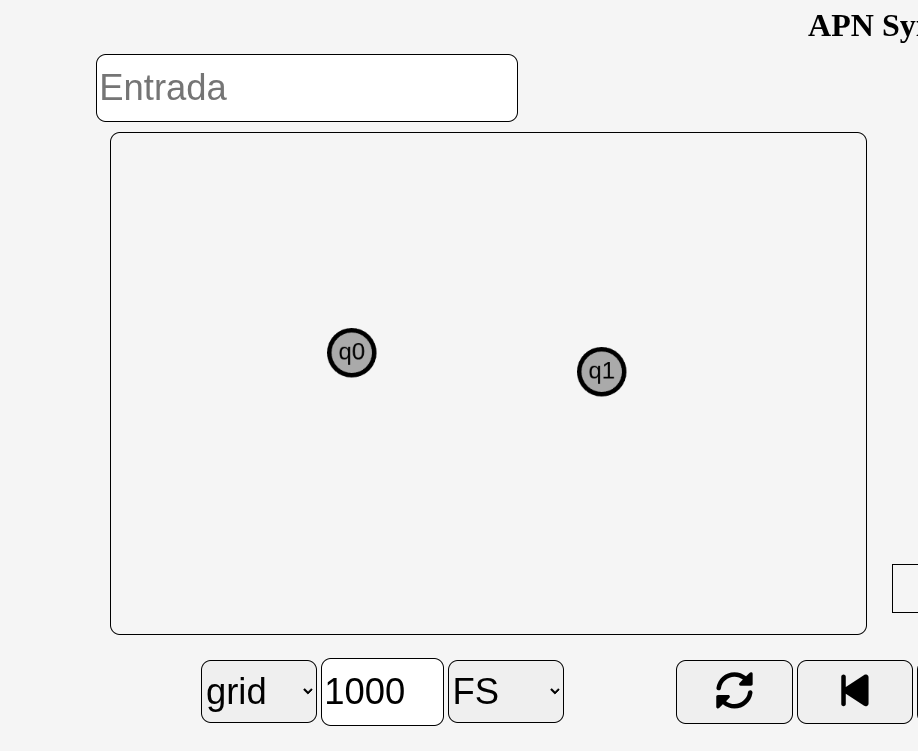
\includegraphics[scale=.24]{img/createState.png}
           \caption{\label{img:createState}}
        \end{subfigure}
        \begin{subfigure}{0.5\textwidth}
           \centering
           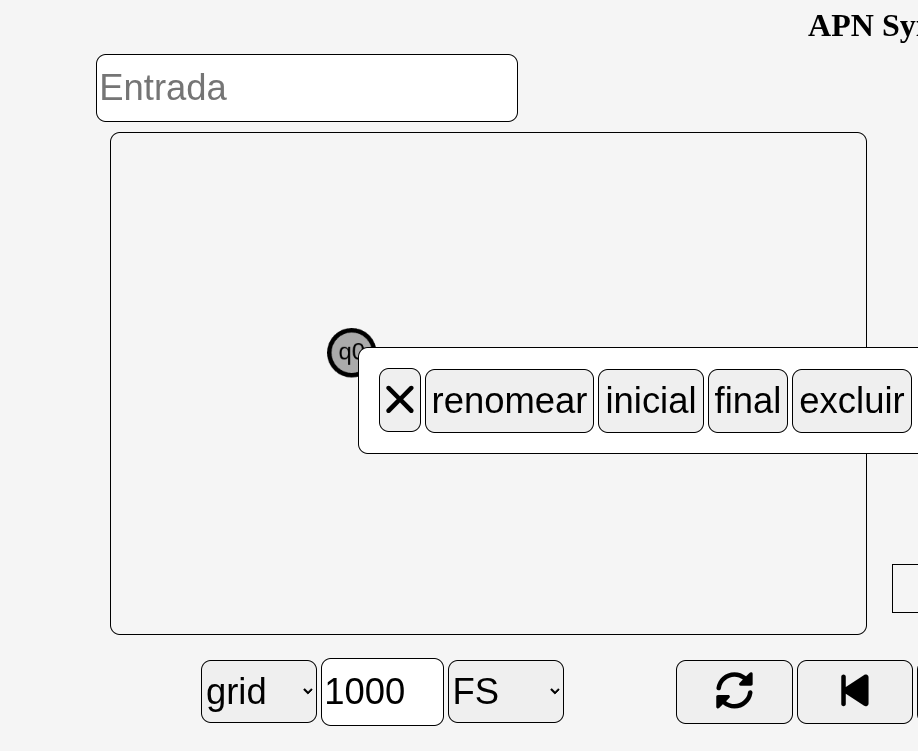
\includegraphics[scale=.24]{img/editState.png}
           \caption{\label{img:editState}}
        \end{subfigure}
        \caption{\subref{img:createState} Criação do estado, \subref{img:editState} Editando o estado }
    \end{figure}

    Para criar uma transição, clique no estado de origem e, em seguida, no estado de destino com o botão esquerdo do mouse. A transição padrão tem o valor vazio em todos os elementos, conforme mostrado na Figura~\ref{img:createTransition}. Ao clicar em uma transição com o botão direito, aparecem suas opções de edição, conforme a Figura~\ref{img:editTransition}, sendo: "excluir", que permite excluir a transição, e "renomear", que permite mudar o carácter de leitura, o carácter a ser desempilhado e o carácter a ser empilhado. Um autômato simples construído na ferramenta pode ser visto na Figura~\ref{img:simpleAPN}.

    \begin{figure}[h]
        \begin{subfigure}{0.5\textwidth}
           \centering
           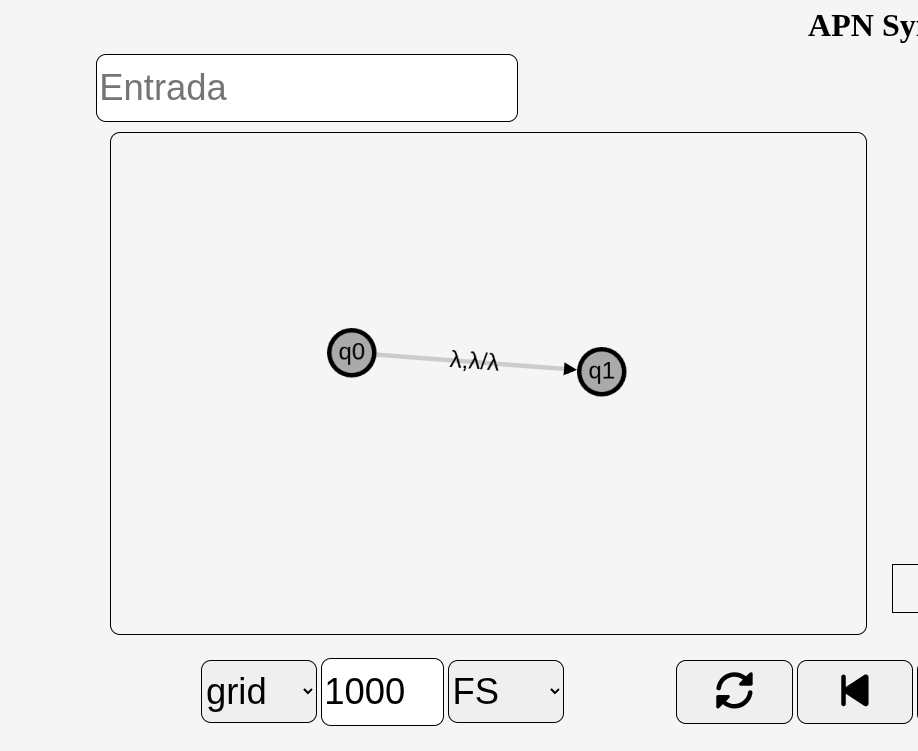
\includegraphics[scale=.24]{img/createTransition.png}
           \caption{\label{img:createTransition}}
        \end{subfigure}
        \begin{subfigure}{0.5\textwidth}
           \centering
           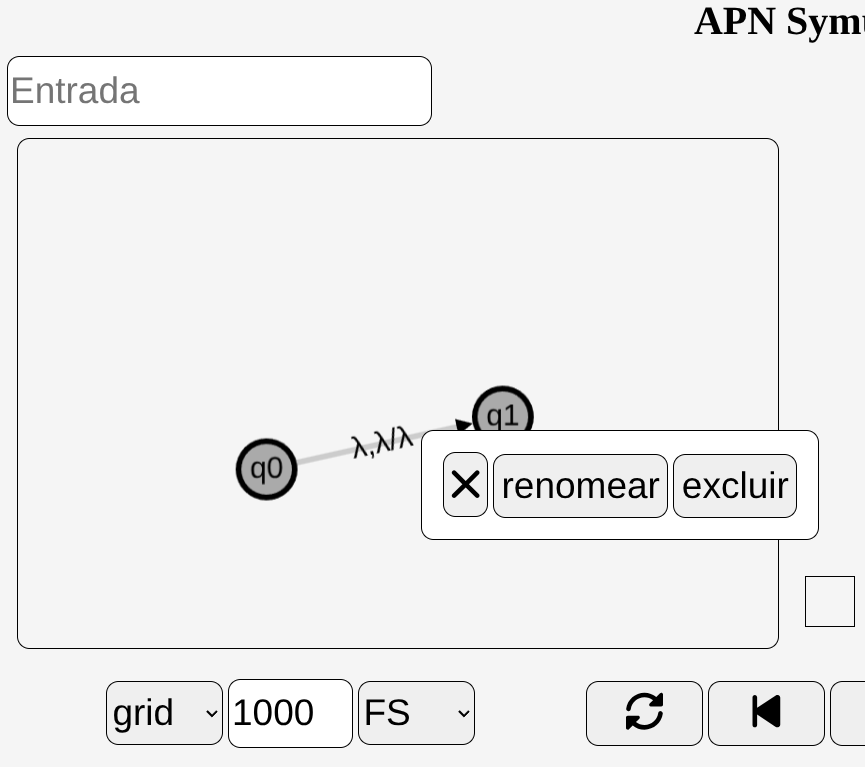
\includegraphics[scale=.24]{img/editTransition.png}
           \caption{\label{img:editTransition}}
        \end{subfigure}
        \caption{\subref{img:createTransition} Criação da transição, \subref{img:editTransition} Editando a transição}
    \end{figure}

    \begin{figure}[] 
        \centering 
        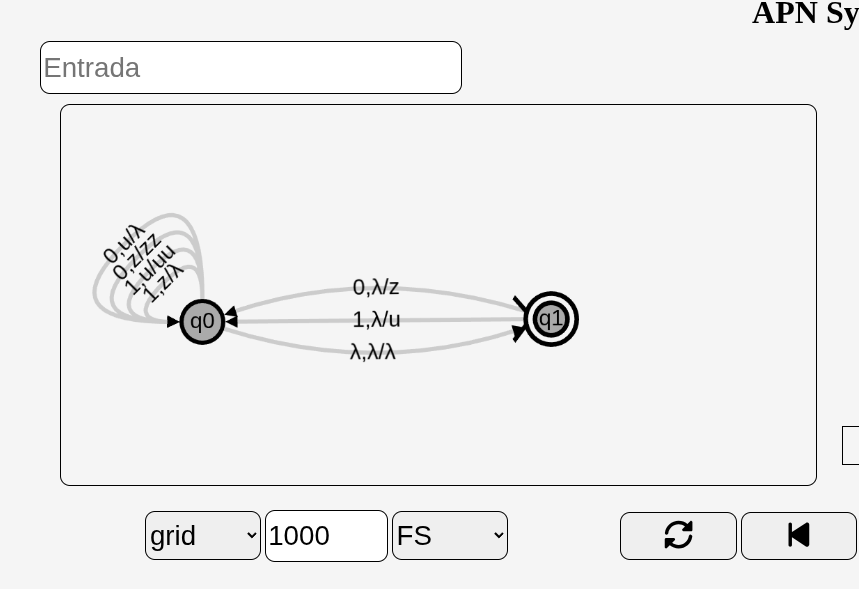
\includegraphics[scale=.24]{img/simpleAPN.png} 
        \caption{Um APN simples} 
        \label{img:simpleAPN}
    \end{figure}

    Ao digitar a palavra de leitura no campo escrito "Entrada", como mostrado na Figura~\ref{img:word0101}, a palavra "0101", e clicar no botão inferior com ícone play, o sistema calcula a execução completa do autômato de acordo com aquela palavra, e o botão de play tem o ícone modificado para stop, que, quando clicado, permite parar a demonstração do autômato com aquela palavra. 

    \begin{figure}[] 
        \centering 
        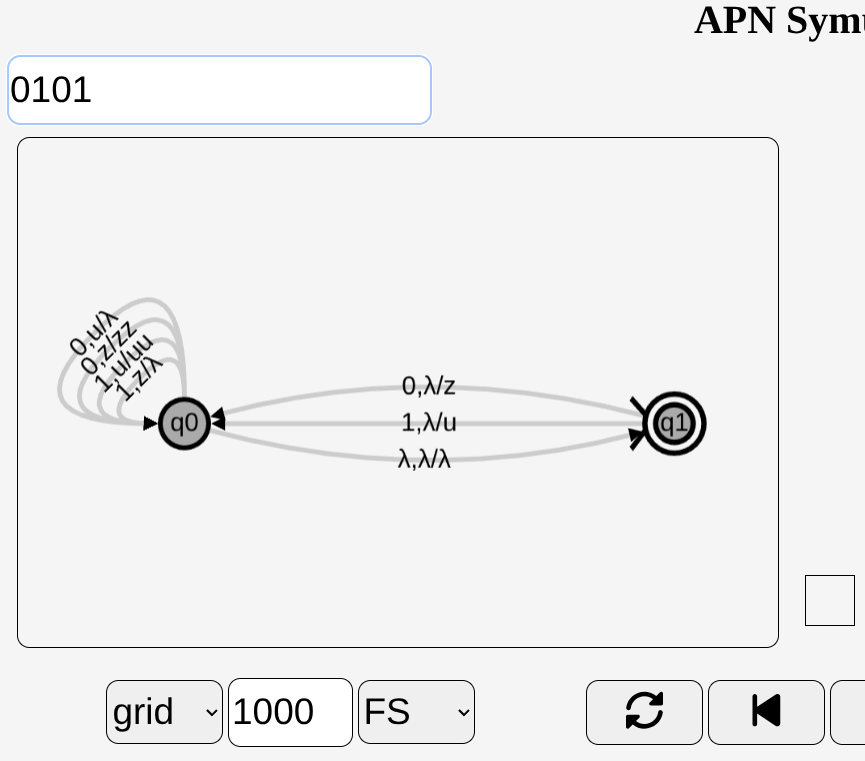
\includegraphics[scale=.24]{img/word0101.png} 
        \caption{entrada de palavra 0101} 
        \label{img:word0101}
    \end{figure}
    
    Durante a execução, é possível ver o campo da palavra substituído por uma tabela com cada caractere e seu índice, destacando o último carácter lido para melhor compreensão, como demonstrado na Figura~\ref{img:wordTable}. Além disso, no painel direito, é possível visualizar cada uma das etapas de execução, chamadas aqui de snapshots, onde aquelas que acabaram de ler o carácter destacado na tabela são destacadas em verde, conforme a Figura~\ref{img:snapGraph}. Em cada snapshot, é possível ver três informações: primeiro, o estado em que ela se encontra no autômato; segundo, o índice do caractere lido na palavra, indicado na tabela; e, por último, os três últimos elementos da pilha desse snapshot.

    \begin{figure}[h]
        \begin{subfigure}{0.5\textwidth}
           \centering
           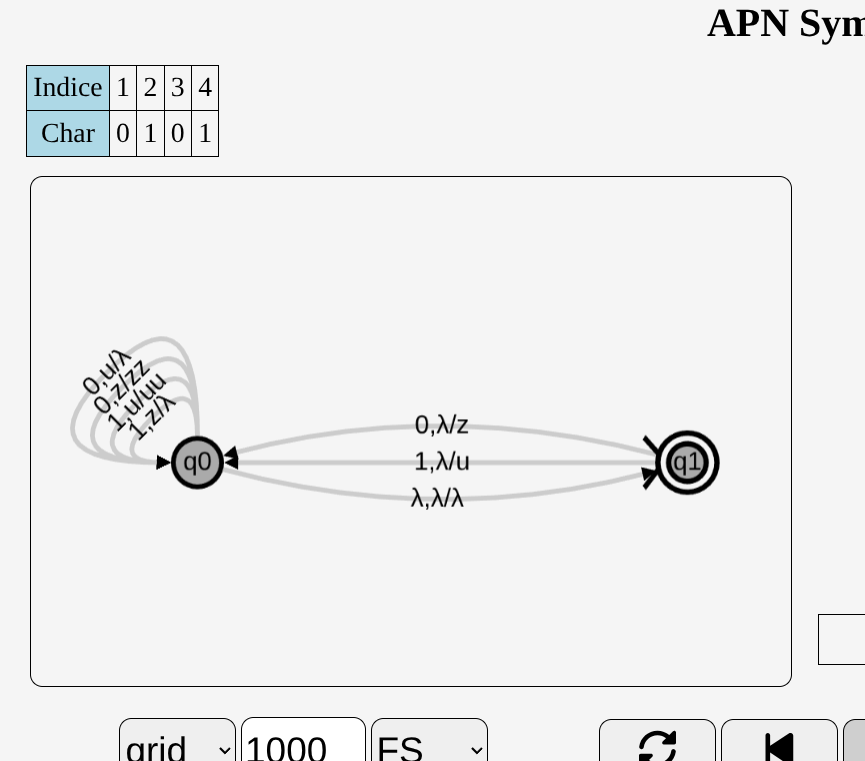
\includegraphics[scale=.24]{img/wordTable.png}
           \caption{\label{img:wordTable}}
        \end{subfigure}
        \begin{subfigure}{0.5\textwidth}
           \centering
           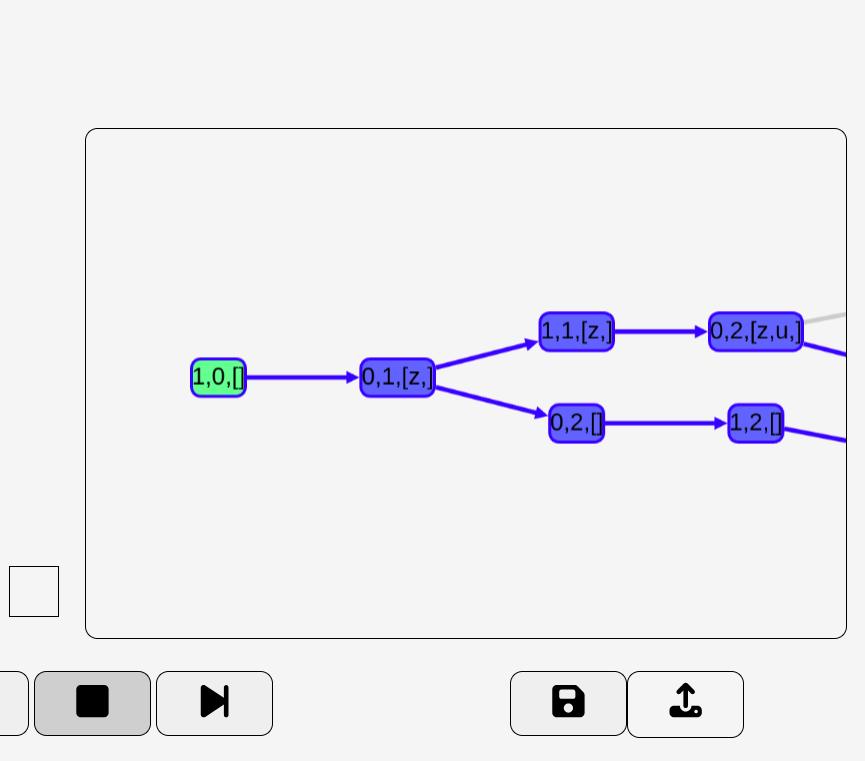
\includegraphics[scale=.24]{img/snapGraph.png}
           \caption{\label{img:snapGraph}}
        \end{subfigure}
        \caption{\subref{img:wordTable} tabela de caracteres, \subref{img:snapGraph} Visualização dos snapshots}
    \end{figure}
    
    No painel direito, as arestas entre snapshots pintadas em azul são aquelas que podem levar a um estado de aceitação conforme mostrado na Figura~\ref{img:acceptedWay}, e as arestas cinzas são as que não levam a um estado de aceitação. Ao clicar em um snapshot, é possível ver sua pilha completa no meio da tela, entre os dois painéis, e ver o estado atual destacado no autômato desenhado no painel esquerdo, conforme a Figura~\ref{img:snapEfect}. Ao clicar no botão com ícone de próximo à tabela da palavra, avança em um caractere, e os snapshots correspondentes são marcados em verde, conforme a Figura~\ref{img:nextButton}, de forma semelhante. Ao clicar no botão com ícone de anterior, é visto o passo anterior de execução.

    \begin{figure}[h]
        \begin{subfigure}{1\textwidth}
           \centering
           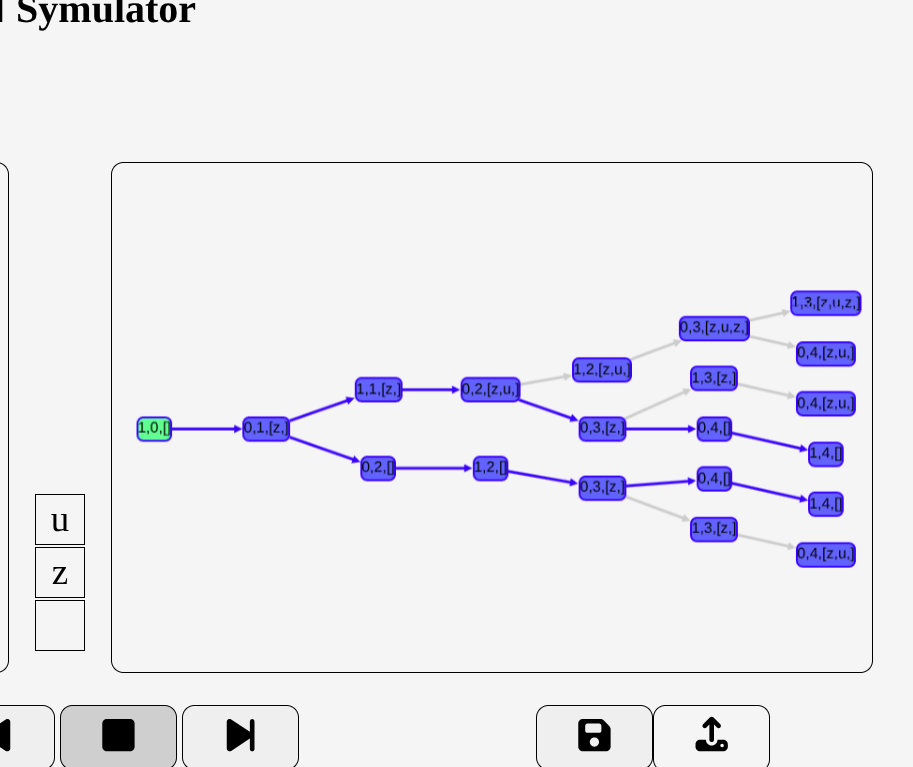
\includegraphics[scale=.24]{img/acceptedWay.png}
           \caption{\label{img:acceptedWay}}
        \end{subfigure}
        \begin{subfigure}{1\textwidth}
           \centering
           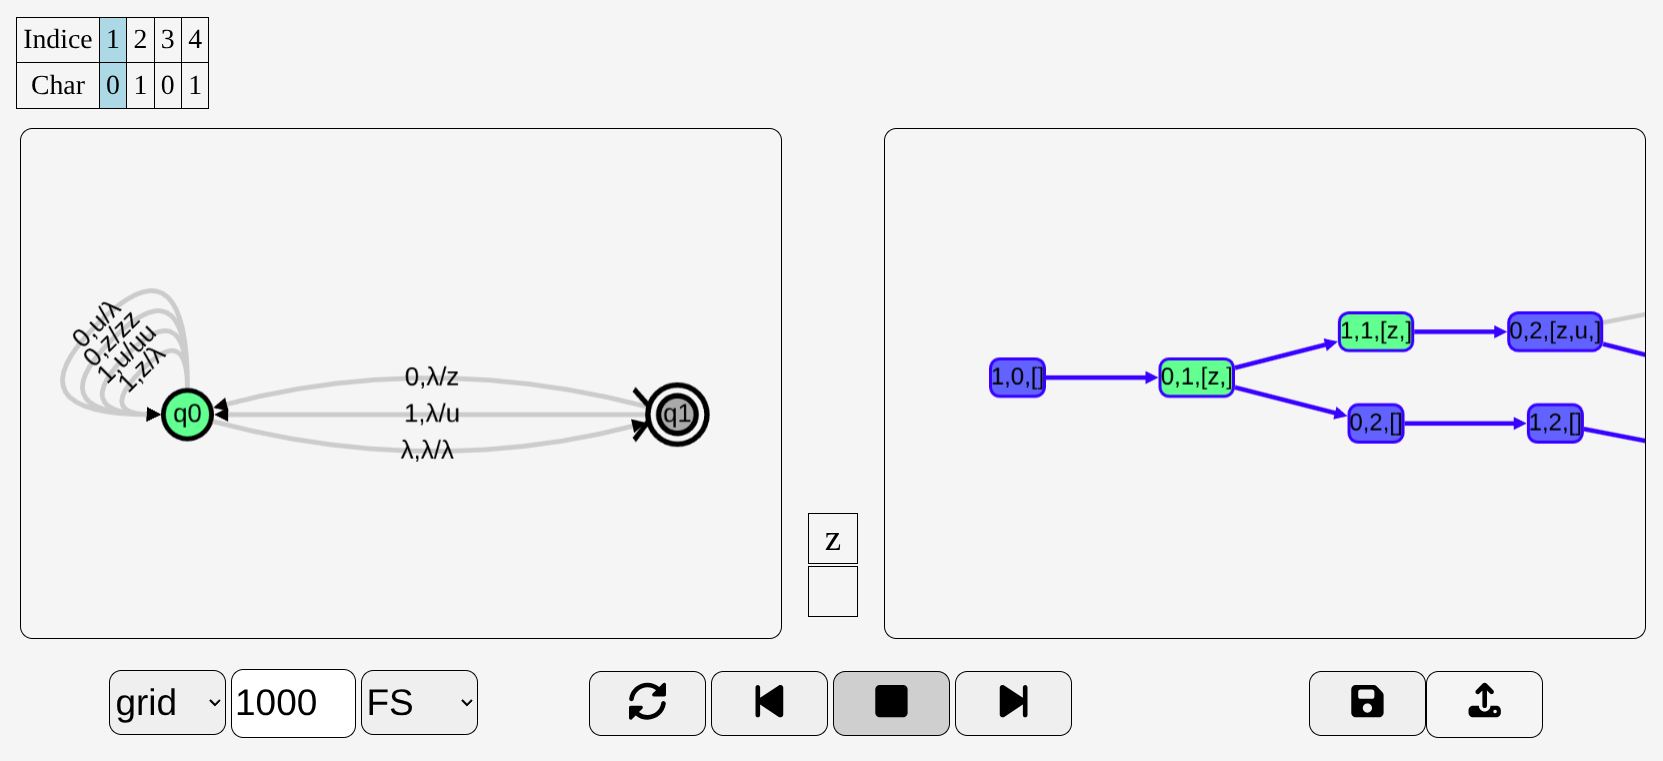
\includegraphics[scale=.24]{img/snapEfect.png}
           \caption{\label{img:snapEfect}}
        \end{subfigure}
        \begin{subfigure}{1\textwidth}
           \centering
           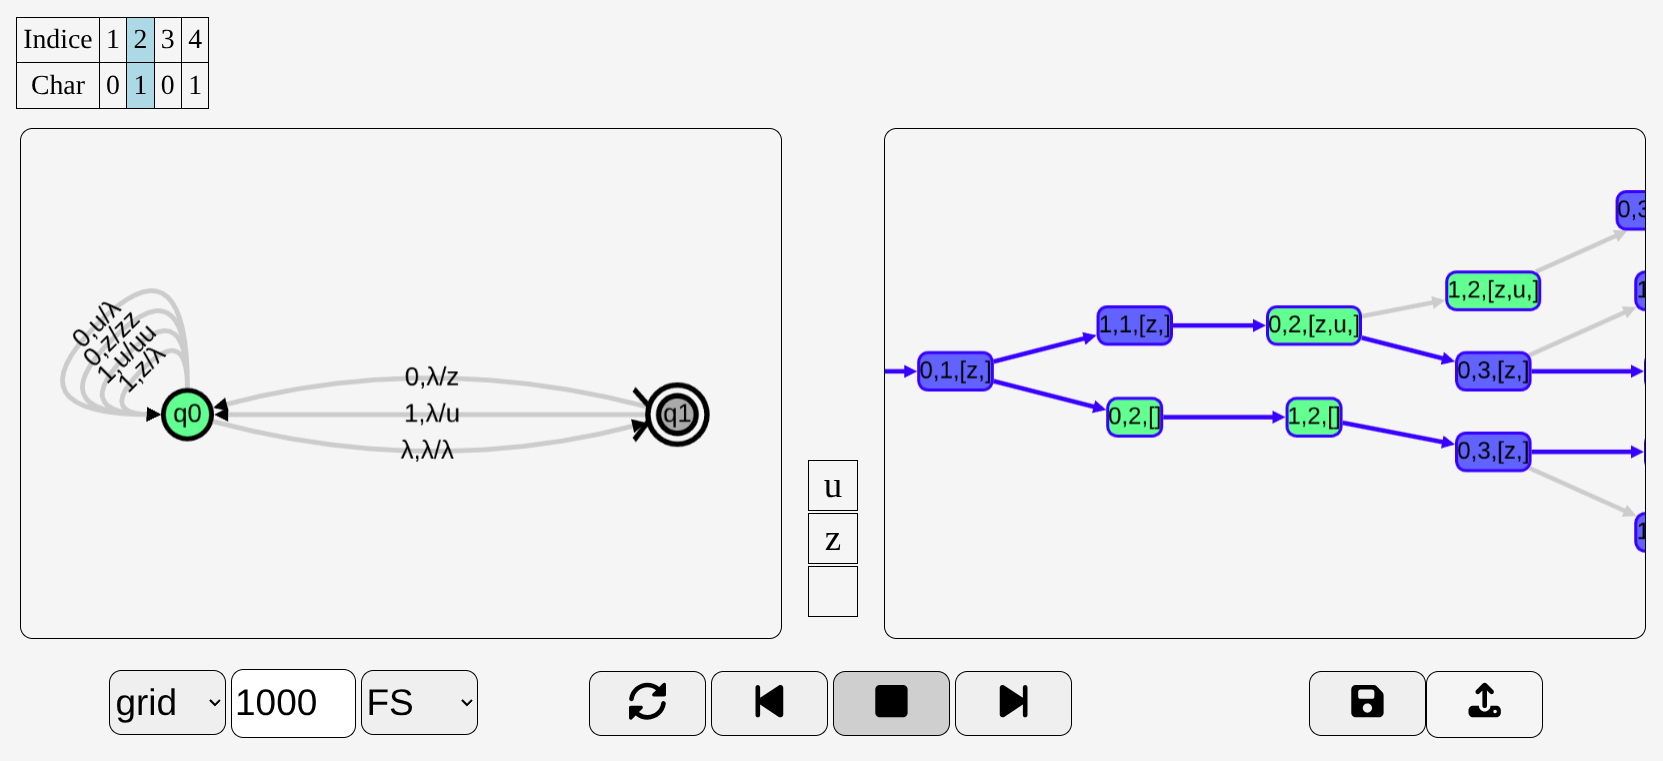
\includegraphics[scale=.24]{img/nextButton.png}
           \caption{\label{img:nextButton}}
        \end{subfigure}
        \caption{\subref{img:acceptedWay} caminho de aceitação, \subref{img:snapEfect} clique em snapshot, \subref{img:nextButton} botão de proximo}
    \end{figure}

    No canto inferior esquerdo, existem 3 botões como mostrado na Figura~\ref{img:configButtons}: o primeiro altera o formato do desenho do APN para o padrão selecionado; o segundo é o limite de loops de execução que esse autômato executa antes de ser forçado a parar; e, por último, o critério de aceitação: FS (estado final e pilha vazia), S (pilha vazia), F (estado final). Por fim,como exibido na Figura~\ref{img:downloadButtons}, existem dois botões no canto inferior direito: o primeiro, com ícone de disquete, serve para fazer download do autômato criado na ferramenta em formato JSON, e o segundo botão, com ícone de seta para cima, serve para fazer upload de um autômato em formato JSON presente no computador do usuário.
    
    \begin{figure}[h]
        \begin{subfigure}{0.5\textwidth}
           \centering
           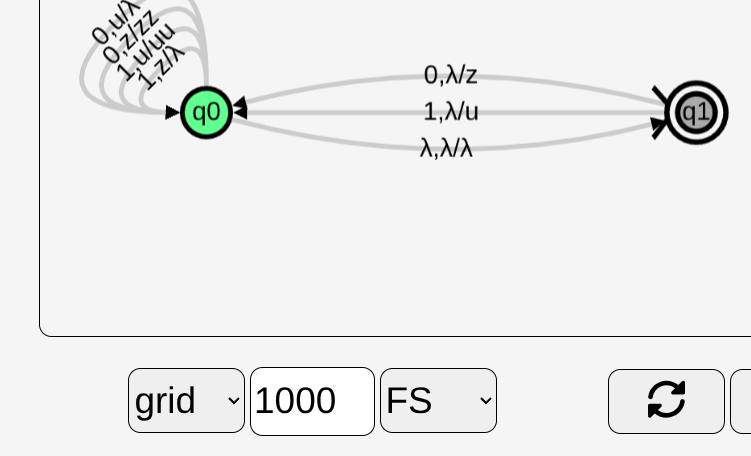
\includegraphics[scale=.3]{img/configButtons.png}
           \caption{\label{img:configButtons}}
        \end{subfigure}
        \begin{subfigure}{0.5\textwidth}
           \centering
           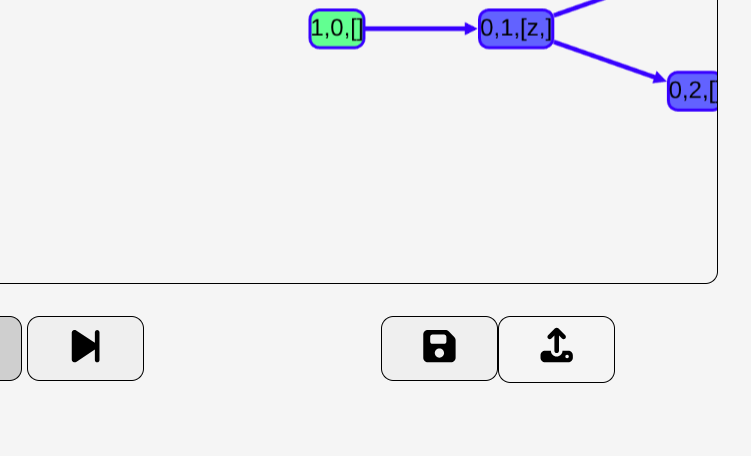
\includegraphics[scale=.3]{img/downloadButtons.png}
           \caption{\label{img:downloadButtons}}
        \end{subfigure}
        \caption{\subref{img:configButtons} botões de configuração, \subref{img:downloadButtons} botões de download}
    \end{figure}
    
